\documentclass[conference]{IEEEtran}

\usepackage{cite}
\usepackage{pslatex} % -- times instead of computer modern, especially for the plain article class
\usepackage[colorlinks=false,bookmarks=false]{hyperref}
\usepackage{booktabs}
\usepackage{graphicx}
\usepackage{xcolor}
\usepackage{multirow}
%\usepackage{flushend} % even out the last page, but use only at the end when there is a bibliography

\newcommand{\code}[1]{{\small{\texttt{#1}}}}

% fatter TT font
\renewcommand*\ttdefault{txtt}
% another TT, suggested by Alex
% \usepackage{inconsolata}
% \usepackage[T1]{fontenc} % needed as well?

\usepackage{listings}

%\newcommand{\todo}[1]{{\emph{TODO: #1}}}
\newcommand{\todo}[1]{{\color{olive} TODO: #1}}
\newcommand{\martin}[1]{{\color{blue} Martin: #1}}
\newcommand{\simon}[1]{{\color{green} Simon: #1}}
\newcommand{\abcdef}[1]{{\color{red} Author2: #1}}
\newcommand{\rewrite}[1]{{\color{red} rewrite: #1}}
\newcommand{\ducky}[1]{{\color{orange} Richard: #1}}
\newcommand{\kasper}[1]{{\color{purple} Kasper: #1}}

% uncomment following for final submission
%\renewcommand{\todo}[1]{}
%\renewcommand{\martin}[1]{}
%\renewcommand{\author2}[1]{}


%%Uncomment the following when you want to add copyright notice and not use any space	 (IEEE only)
%\usepackage[absolute]{textpos}
%% Set unit to be pagewidth and height, and increase inner margin of box
%\setlength{\TPHorizModule}{\paperwidth}\setlength{\TPVertModule}{\paperheight}
%\TPMargin{5pt}
%% Define \copyrightstatement command for easier use
%\newcommand{\copyrightstatement}{
%	\begin{textblock}{0.85}(0.072,0.93)    % Tweak here: {box width}(leftposition, rightposition)
%		\noindent
%		\normalsize
%		???-?-?-???-?/??/\$31.00~\copyright20?? IEEE % Put here your copyright
%	\end{textblock}
%}

\begin{document}


%\title{Towards Verification of Digital Circuits with\\
%SystemVerilog/UVM and Chisel/Scala}

\title{Towards an Open-Source Verification Method with\\
Chisel and Scala}

\author{\IEEEauthorblockN{Martin Schoeberl, Simon Thye Andersen,\\ Kasper Juul Hesse Rasmussen, Jan Madsen}
\IEEEauthorblockA{\textit{Department of Applied Mathematics and Computer Science} \\
\textit{Technical University of Denmark}\\
Lyngby, Denmark \\
masca@dtu.dk, simon.thye@gmail.com,\\ s183735@student.dtu.dk, jama@dtu.dk}
\and
\IEEEauthorblockN{Richard Lin}
\IEEEauthorblockA{\textit{Department of Electrical Engineering and Computer Sciences} \\
\textit{UC Berkeley}\\
Berkeley, CA \\
richard.lin@berkeley.edu}
}
% Most conferences have their own commands for author headings.

%\author{\IEEEauthorblockN{Edgar Lakis, Martin Schoeberl}\\
%\IEEEauthorblockA{Department of Applied Mathematics and Computer Science\\
%Technical University of Denmark\\
%Email: \texttt{edgar.lakis@gmail.com}, \texttt{masca@imm.dtu.dk}}
%}


\maketitle \thispagestyle{empty}

\begin{abstract}

\end{abstract}

\begin{IEEEkeywords}
digital design, verification, object-oriented programming
\end{IEEEkeywords}

\martin{We aim for \url{https://woset2020.hotcrp.com/}}

\section{Introduction}
\label{sec:intro}


Performance increase with general-purpose processors came to a halt.
We cannot longer depend on Moor's Law to increase computing performance~\cite{dark-silicon:2011}.
The only way to achieve higher performance or lower energy consumption
is by building domain-specific hardware accelerators~\cite{domain-hw-acc:2020}.
To efficient develop those accelerators we can learn from software development trends
such as agile software development. We need agile hardware development~\cite{henn-patt:turing:2019}.


\martin{does not like this abstract.}
Production of a chip is very expensive. Therefore, it is important to get the design right
at the first tape-out. Throughout testing and verification of the design is mandatory.
Until a few years, the two main design languages Verilog and VHDL dominated the
design and testing of digital circuits. However, both languages are decades behind
modern languages for software development. \ducky{Why? What is great (and what do we want to bring over) from SW dev? Remember that SW is cheap and easy to change (so it's worth it to have bugs but ship faster), so it's not necessarily an apples-to-apples comparison.}

Resent advances with SystemVerilog and Chisel \ducky{should probably be described} bring object-oriented programming
into the digital design and verification process. SystemVerilog, as an extension of Verilog,
adds object-oriented concepts for the non-synthesizable verification code.
Chisel is a language, embedded in Scala, to describe digital circuits.
Circuits described in Chisel can be tested and verified with a Chisel testing
framework and tests written in Scala.
Scala/Chisel brings object-oriented and functional programming into the world of
digital design. \ducky{What about OOP is great? How specifically does it benefit HW dev? Note, in SW dev, OOP can be done wrong / badly / verbosely (eg, Java), while (one of) the ASPIRE / ADEPT arguments for Chisel is generators + re-use.}

This paper describes a research project that aims at building a testing framework
in Scala that takes the best methods from UVM and from decades of experience
in software testing.

\ducky{Chisel is a synthesis language, without dedicated test constructs - do one thing well, instead of the jack-of-both-trades Verilog/SystemVerilog}
\martin{Ok, fixed it.}

\todo{A brief introduction what the paper is about. It shall include briefly the
main contributions and findings. The contributions can be bullet listed.}

This paper... \todo{purpose statement, latest in 4th paragraph}

\todo{Test the bib with a reference that gives background on time-predictable
computer architecture~\cite{tpca:jes}.}

A paper is cited \cite{paper:example}.

The contributions of this paper are: (1) ... (2) ...

This paper is organized in N sections: The following section presents related work.
Section~\ref{sec:related} provides background on the Universal Verification Methodology ...
Section X and Y 
Section~\ref{sec:eval} evaluates...
Section~\ref{sec:conclusion} concludes.


\section{Overview of the Universal Verification Methodology}
\label{sec:related}


\todo{Related to our work}

\todo{reference for UVM}

The Universal Verification Methodology (UVM) is a methodology for testing and verification of digital circuits, introduced in 2011. Previously, verification methodologies were vendor-specific, forcing users to stay with one tool, or to spend a lot of time and money transitioning to a new tool. UVM is unique in the fact it is an Accellera standard developed together with all of the major EDA vendors such as Questa, Cadence and Synopsys. As of 2017 it has also been standardized as IEEE 1800.2. Although SystemVerilog and UVM are IEEE standards, the standards are freely available from the IEEE.

UVM is implemented as a SystemVerilog library, and utilizes the fact that SystemVerilog allows for object-oriented design of testbenches. By using OOP patterns such as inheritance and polymorphism, the verification engineer is able to design generic components that can be extended and modified to provide application-specific functionality. 

\subsection{A UVM Testbench}
UVM Testbenches consist of several distinct components, as seen in Figure~\ref{fig:uvm_testbench}. Each component performs only one task in the testbench, allowing the engineer to make changes to some components without affecting others. 
For example, the sequencer is the component responsible for generating transactions for the DUT, whereas the driver is responsible for converting the transaction into pin-level wiggles, i.e. generating correct start/stop conditions as well as driving signals. If a new sequence of transactions is to be generated, only the sequencer is affected. Likewise, the sequencer does not care in what way the transactions are converted into pin-level signals - this is the sole responsibility of the driver. This makes for easier testbench design as there are fewer unnecessary dependencies. 

\begin{figure}
    \centering
    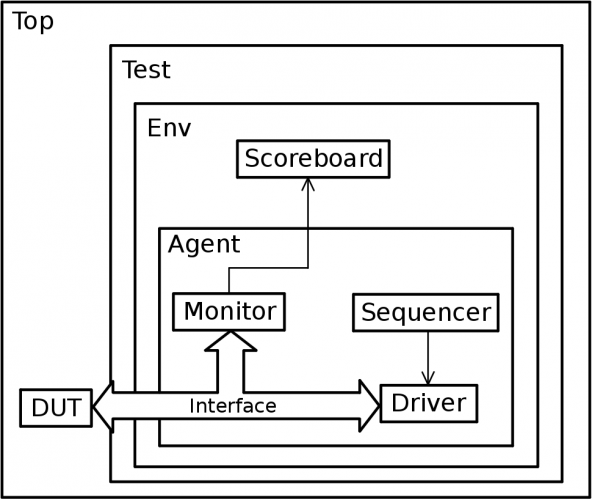
\includegraphics[width=0.475\textwidth]{uvm-tb_Pedro-Araujo.png}
    \caption{Representation of a simple UVM testbench. By Pedro Araújo / colorlesscube.com}
    \label{fig:uvm_testbench}
\end{figure}

\ducky{an alternative graphic might be a layered (think networking, eg, TCP/IP or OSI model) graphic}

The main components of a UVM testbench are as follows
\kasper{Is this necessary? I had a difficult time understanding why all of the different components were necessary at first, but people with more verification experience might find it too basic?}
\ducky{I think what this really needs (if this is needed at all) is an example that explains how all the parts work together, and what role they play in a whole testbench. The general argument for this is separation of concerns - it's not a great fit for small-scale testbenches like a single ALU, but makes more sense when working with complex systems and protocol buses. In a sense, it makes hard things easier, and easy things unnecessarily cumbersome - so does not scale down gracefully.}
\begin{itemize}
    \item \textbf{Sequence(r):} Sequences define the order of transactions necessary for a given purpose, e.g. a synchronisation or reset sequence. The sequencer is responsible for transferring the transactions, defined by the sequence, to the driver
    \item \textbf{Driver:} Converts transactions into pin-level signals and drives these signals onto the DUT
    \item \textbf{Interface:} Interfaces are a SystemVerilog construct which allow the user to group related signals. A DUT may have several interfaces attached. The interface is used to avoid hooking directly into the DUT. 
    \item \textbf{Monitor:} Monitors all traffic on the interface, converting pin-level signals into transaction-level objects that can be operated on by other components, such as a coverage collector or scoreboard. 
    \item \textbf{Agent:} Encapsulates monitor, sequencer and driver, setting configuration values. Agents may be set active or passive (with or without a driver and sequencer). Useful when it is necessary to have multiple instances of the same components, e.g. when a 4-port network switch needs four identical drivers
    \item \textbf{Scoreboard:} Is used to check whether correct functionality is achieved. Usually does so by use of a golden model / co-simulation via the SystemVerilog Direct Programming Interface
    \item \textbf{Environment:} The environment is used to configure and instantiate all child components. Environments are typically application-specific, and may be modified by the test
    \item \textbf{Test:} The test is the top-level verification component. The test designer may choose to perform factory overrides of classes and set configuration values here, which modify the child components
\end{itemize}

As can be seen above, even a "Hello, World" example using the UVM requires that the user understands how and why each of the different UVM components should be used. This causes UVM to have a very steep learning curve which may discourage adoption. However, once the initial setup of the testbench has finished, expanding its functionality becomes easier.


\martin{Does BluseSpec Verilog has something to offer?}
\ducky{BSV is a higher-level design abstraction around guarded atomic actions - so relevant in terms of raising the level of design for digital logic, but a different approach than Chisel. My understanding (which may be outdated / wrong) is that BSV is propreitary, which is one reason it does not have significant traction. Earlier versions were heavily Haskell-based, which also does not help with perceived usability, supposedly that is why they're now branded "Bluespec SystemVerilog".}

\section{The Open-Source Tools}

\subsection{Chisel}

Chisel is a hardware construction language in Scala.~\cite{chisel:dac2012}.
Chisel allows the user to write hardware generators in Scala, which itself is an object-oriented and functional language. For hardware generation and testing, the full Scala language and Java
libraries are available. For example, we read in the string based TDM
schedules~\footnote{available at: \url{https://github.com/t-crest/s4noc/tree/master/noc/vhdl/generated}}
and convert them with a few lines of Scala code into a hardware table to
drive the multiplexer of the router and the NI.

Chisel is solely a Hardware Construction Language, and thus all valid Chisel code maps to synthesizable hardware. By separating the hardware construction and hardware verification languages, it becomes impossible to write un-synthesizable hardware and in turn speeds up the design process. As the full power of Scala and Java is available to the verification engineer, the verifcation process is also made more efficient.

\martin{This is just a starting point, way more is needed.}

\subsection{ChiselTest}

\martin{Richard should write}

\cite{chisel:tester2}

\subsection{Simulators}

\todo{On Treadle and Verilator}

\martin{Maybe a few words from Richard on Treadle, Simon on Verilator?}



\subsection{Scala}

The test environment and the driving code is written in Scala. Scala with its
compatibility with Java has a very rich open-source library ecosystem.
If you need a tool, e.g., and ELF file reader to load a binary, there will be a Java
library available for it.

Furthermore, we can use all the testing libraries that have been developed for
software development. A popular library is ScalaTest. A Chisel tester can be embedded
in a ScalaTest components and a simple \code{sbt test} will execute all the tests.

\todo{Check what ScalaCheck can offer.}

\section{Integrating Legacy Languages}

A verification method is only usable when it can handle mixed-source designs.
This means a Scala driven method mast be able to test components written in Verilog,
VHDL, and SystemVerilog.

\subsection{Verilog Components}

\todo{write on black boxes and Verilator}

\subsection{VHDL Components}

Chisel has support for black boxes, which allows the use of Verilog code within the Chisel design. However, it does not fully support VHDL. It can support VHDL using VCS, but there is no open source solution available for VHDL. This is due to the use of Treadle and Verilator \simon{Ref} for open source simulation. Treadle only supports Chisel code while Verilator is run on the generated Verilog. Therefore, Verilator can also simulate black boxes written in Verilog. However, VHDL is now a concern to companies that have a lot of source code written in VHDL, which needs to be compatible with any systems written in Chisel. As many simulation and synthesis tools support mixed-language implementations, this is not an issue for the implementation part. But for open source testing, it proves to be a problem.

A solution for this is based on the principle of using synthesis tools to analyze the VHDL RTL code and synthesize a gate-level netlist for this. These synthesis tools can often output a Verilog-based netlist. A free solution for this would be the Yosys \simon{ref} synthesis suite, which is an open-source digital hardware synthesis suite for Verilog code. It has support for VHDL by using Verific as a front-end, which requires a license. For an alternative solution to this, GHDL \simon{ref} would be used. GHDL is an open source simulator for VHDL which also funcions as a plugin for Yosys. This allows yosys to analyze VHDL files using GHDL and then synthesize a circuit. The gate-level netlist can then be saved as a Verilog file, which can be used for the simulation system. GHDL has full support for IEEE 1076 VHDL 1987, 1993, 2002 and a subset of 2008.

Testing
\simon{Insert small image that depicts the workflow for this.}

\section{First Experiments}

Although this is a work-in-progress report, we have started with an evaluation.
A simple ALU has been implemented in SystemVerilog, classic Verilog, VHDL, and Chisel.
We wrote a testbench in SystemVerilog / UVM and in Scala. As execution platform we used Synopsys VCS, ModelSim, Treadle, and Verilator.
\ducky{Likely criticism from peer review is that the example is too simple.}
\ducky{I'd also like to see some kind of human evaluation - though I'm not sure what kind of methodology is accepted in the digital design community. Could maybe drop a HCI paper cite to hint that whatever methodology used is accepted in other communities.}

\martin{We could also use my NoC example, which is not trivial ;-)}

The examples are available in open source from: \url{https://github.com/chisel-uvm/chisel-uvm}.

\subsection{Using UVM with Chisel}

The Chisel toolchain translates Chisel code into plain Verilog for simulation and synthesis. Therefore, we can use a UVM based test bench to test Chisel generated code.
An important issue is that the modules and port names in the generated Verilog code are reasonable and do not change when changing the Chisel design.

A UVM testbench has been designed to test the various implementations of the reference design, a simple ALU from the Leros project \cite{leros:fpl2011}. Functional coverage is being collected on the following parameters.
\begin{itemize}
    \item All operations have been performed
    \item All operations have been performed after a reset
    \item A number of "interesting" values are tested (-32768, -1, 0, 1, 32767)
\end{itemize}

In addition, a scoreboard is used to verify the functionality of the DUT. The reference model is modelled as a SystemVerilog case statement, as the DUT is only an ALU and no state information is required.

As a SystemVerilog interface is used, no details about the DUT are exposed to the driver and monitor. This makes it easy to replace the DUT with an alternative implementation, e.g. in another HDL, and verify its functionality. It is only necessary to instantiate the new DUT and connect it to the interface, after which the test can be run.

The UVM testbench has been run on the Verilog description generated by Chisel, as well as a VHDL version of the ALU. Using the VHDL version required more manual work to make the mixed-language simulation work, whereas the Verilog version was very fast to implement. Generating Verilog with Chisel and testing with UVM then proves to be a suitable workflow if an open-source SystemVerilog simulator with UVM support is used. \todo{Does Verilator support SystemVerilog / enough SV to also support UVM?}

\section{The Road Ahead}

\todo{ScalaTest and PBT with ScalaCheck.}


\subsection{Source Access}

\martin{I love doing papers with available source under an
open-source license. It gives credit and good karma.}


\section{Conclusion and Future Work}
\label{sec:conclusion}

This work-in-progress paper is a first sketch of the ideas to combine SystemVerilog/UVM
with Chisel/Scala for a productive design and verification of future digital circuits.
We will explore all combinations with a few small examples, provided by our industrial
partners.
From that we will bootstrap adding constraint-random verification methods to Chisel
testers and collecting coverage metrics within FIRRTL.

\subsection*{Acknowledgment}

\todo{Sometimes we received some help. Sometimes external funding.}

%This work was partially funded under the
%European Union's 7th Framework Programme
%under grant agreement no. 288008:
%Time-predictable Multi-Core Architecture for Embedded
%Systems (\mbox{T-CREST}).

%\newpage


\bibliographystyle{plain}
% Please do not add any references to msbib.bib.
% They get lost when I 'generate' is again (see Makefile)
\bibliography{chisel-uvm,msbib}

\end{document}
~
\newpage
~
\newpage

\section{The Classic Hardware Description Languages}

\section{SystemVerilog}

\todo{adds some VHDL features to Verilog. Tries to please VHDL developers.}

SystemVerilog is IEEE standard, proprietary tools.

Chisel is research stuff and open-source

\section{Chisel}

Chisel~\cite{chisel:dac2012} 

\section{Combining the Approaches}

Although SystemVerilog/UVM and Chisel/Scala look like competing initiatives
to solve the verification problem, it should be possible to combine those two methods.
By using this combination we might be able to enjoy the benefits of both worlds:
the industrial proven SystemVerilog/UVM tool chain with the available IPs with
the research and more software oriented approach of Chisel/Scala. 

\todo{Be nice to all and show how we can combine different approach to
get the best of both worlds}

\ducky{The main nontechnical benefits of UVM are a large library and userbase, and this inertia is probably going to hamper adoption of a new tool, especially if that new tool is more incremental than revolutionary. To my understanding, the main technical benefits of UVM are re-use and separation of responsibilities, and is inspired by an old-ish (and fairly verbose) form of OO}

\subsection{Using UVM with Chisel}

The Chisel toolchain translates Chisel code into plain Verilog for simulation and
synthesis. Therefore, we can use a UVM based test bench to test Chisel generated code.
An important issue is that the modules and port names in the generated Verilog
code are reasonable and do not change when changing the Chisel design.

\subsection{UVM with VHDL}
\kasper{Shouldn't this actually be UVM with (System)Verilog? Or are we focusing specifically on VHDL because UVM isn't made for VHDL, and thus we're looking into what's possible?}
\martin{One can also use UVM/SystemVerilog test logic with a VHDL DUT.}

\subsection{Chisel with Verilog}

\subsection{Chisel with VHDL}

\subsection{Chisel with UVM}

\todo{reusing Chisel tests (ScalaTest) within the UVM framework
with the generated Verilog code}
\ducky{UVM is largely a framework and library for testing blocks ("IP"), I don't think transpiling ChiselTest to UVM is feasible. Best I would practically hope for is interop between both, eg ChiselTest hooks to call UVM functions in a Verilog simulation environment, to enable continued use of legacy test code, Not sure the other way around is worth doing (calling ChiselTest functions from within a UVM environment)}

\section{Co-Simulation}

\todo{with C/C++/Java/Scala/Phyton, ....}
\ducky{Should be tons of this already. CoCoTb is a Python cosimulation environment. Rocket-chip uses C++ cosimulation in their RTL tests.}


\section{Notes}

Here collect of notes and ideas in bullet list for the development and writing process:

\begin{itemize}
\item Collect related work
\item Some more notes
\end{itemize}

\subsection{Comparison}

\begin{itemize}
\item UVM is directly supported in major tools
\item UVM is based on SystemVerilog (SV)
\item OO in SV is only for test benches, not for HW description
\item SystemVerilog is three languages in one: old Verilog, new SystemVerilog for synthesize
(what constructs are supported by what tool), and SV for test benches
\item SV is a specialized language for HW design and testing
\item Chisel is two languages: Chisel for HW and Scala for tester
\item Chisel supports OO for HW description
\item Chisel is based on Scala
\item Scala is a general purpose languages
\item Scala/Chisel can use Java libraries (a LOT is available)
\item Number of Scala programmers are larger than SV programmers (how much?)
\item UVM is open source
\item SV implementation is closed source, needs commercial tools
\item UVM/SV is available on EDAPlayground
\item Chisel/Scala is open source
\item Chisel/Scala runs on the JVM, on Windows, Linux, and macOS
\item Chisel is missing the UVM methodology
\item SV (tools) supports coverage, Chisel does not
\item UVM provides functions for random constraint testing, Chisel/Scala not
\item UVM has a lot of IPs available (e.g., AXI)
\item Chisel testers need some library for sequencing and interfacing (bachelor/master thesis on parts)
\item Verdi is a GUI with knowledge of UVM
\item Verilator with C/C++ emulation is another verification option
\end{itemize}

\subsection{Research Questions}

\begin{itemize}
\item Can we use Chisel testers within UVM?
\item Can we run JVM based code in UVM?
\item Doing UVM verification on Chisel generated Verilog
\item UVM testing on Chisel interpreter (like Chisel tester using treadle, or Verilator)
\end{itemize}

\subsection{Big Research Questions}

These topics are probably good questions for a larger research project.
Part of this is probably already looked at by PhD students at UCB.

\begin{itemize}
\item Add coverage to Chisel tester
\item Provide random constraint functions
\item Provide UVM functions
\item 
\item 
\end{itemize}

\subsection{Helpful links and resources}

VHDL/SV comparison: \url{http://www.sunburst-design.com/papers/CummingsSNUG2003Boston_SystemVerilog_VHDL.pdf}

Open-source design flow, maybe for the Basys3: \url{https://symbiflow.github.io/}

Video primer on using UVM, explains what each component of the UVM test does and why things are set up the way they are
\url{https://www.youtube.com/watch?v=FkclDiK4Oco}

Website that has relatively in-depth and understandable explanations of UVM concepts and structure
\url{https://www.chipverify.com/uvm/uvm-hello-world}






\end{document}

%% Adding a comment to test linking with overleaf
